\documentclass[10pt,a4paper]{article}
\usepackage[margin=1.7cm]{geometry}
\usepackage{graphicx}
\usepackage{parskip}
\usepackage{float}

\title{\vspace{-1.5cm}Predicting Soil Texture from VisNIR Spectra}
\author{Nedjar Abdelmalek}
\date{10 September 2026}

\begin{document}
\maketitle

\section{Introduction}

Soil texture is the amount of sand, silt and clay in a soil. It controls how much water the
soil can hold, so it matters for farming and for soil carbon. Today, texture is measured in a
laboratory. This is slow and expensive, so we cannot do it for every field.

Reflectance spectra are much faster to measure. If a model can predict texture from a
spectrum, we can measure many more soils. And if the model still works with satellite bands,
we could map soil texture over large areas.

In this lab I answer three questions. Can I predict sand, silt and clay from a laboratory
spectrum? How much do I lose when the spectrum is reduced to what a satellite really sees?
And does the model still work on a survey it has never seen? The third question turned out to
be the most important one.

\section{Data}

The data comes from the Open Soil Spectroscopy Library (OSSL). It has \textbf{40\,535
samples}. One row is one soil sample measured in a laboratory, with its spectrum.

Each row has 421 reflectance values, from 400 to 2500 nm, one every 5 nm. It also has the
three targets (sand, silt and clay), the sampling depth, the position, the instrument, and
the programme. The three programmes are LUCAS.SSL (22\,171 samples), KSSL.SSL (14\,728) and
ICRAF.ISRIC (3\,636).

The three targets already sum to 100 for every sample (minimum 99.9999, maximum 100.0001).
So only two of them are free.

\textbf{What I removed and why.}

\begin{itemize}
\item \textbf{The wavelengths 400 to 450 nm (11 columns).} They are missing for all 22\,171
      LUCAS rows, because the XDS instrument starts at 455 nm. This is not random: it is one
      instrument. I use the 410 columns from 455 to 2500 nm for every model.
\item \textbf{Two rows with dead spectra.} Their reflectance is exactly 1.0 at all 421
      wavelengths. These are failed measurements. Their texture values are normal, so no
      filter on the targets would find them.
\item \textbf{Band B1 and 5 hyperspectral bands.} Their windows are inside the missing block,
      so they are NaN for LUCAS. I keep 11 of 12 satellite bands and 170 of 175.
\item \textbf{498 rows without coordinates.} I removed them only for the map (task 1.12).
\end{itemize}

One important property of this data: \textbf{the programme is also the instrument, the region
and the sampling depth}. Each programme used exactly one instrument, in one part of the
world. The mean reflectance is 0.65 for LUCAS and 0.40 for the two others. So when I remove
one programme from training, all of these change at the same time.

\section{Methodology}

\textbf{Sensor simulation.} I built two simulated sensors. The first has the 12 bands given
in the lab sheet. The second has 175 bands, each 12 nm wide, every 12 nm from 400 to 2500 nm.
For each band I take the simple mean of every laboratory wavelength inside
$\mathrm{centre} \pm \mathrm{width}/2$. This is a rectangular spectral response. If any
wavelength inside the window is missing, the band is NaN.

I chose this rule because it only needs the band table from the sheet, and it keeps the
averaging that makes a wide band useful. Each band averages between 3 and 37 readings. I
rejected a Gaussian response weighted by FWHM, because the real curves were not given. I also
rejected taking the single nearest wavelength, because it loses the averaging.

\textbf{Model.} I used PLS regression, with one model per target. Neighbouring wavelengths
correlate at 0.999944, so normal regression would be unstable. PLS uses a few latent
components instead. I fixed the number of components (20 for the full spectra, 10 for the 11
bands) and I did not tune it. This way the results compare the versions of the spectra, and
not the tuning effort.

\textbf{Evaluation.} I used two schemes. The first is a random 80/20 split. The second trains
on two programmes and tests on the third, repeated for each programme. The random split puts
samples from the same survey on both sides. Because the surveys have different brightness, the
model can recognise the survey and use its average texture. Leaving a programme out removes
this shortcut.

\textbf{Explainability.} I used two methods on the clay model. Permutation importance shuffles
one wavelength and measures how much $R^2$ falls. VIP measures how much each wavelength
contributes to the components PLS built. I ran the first method with three seeds, and I also
shuffled whole 20 nm blocks instead of single wavelengths.

\section{Results}

\begin{figure}[H]
\centering
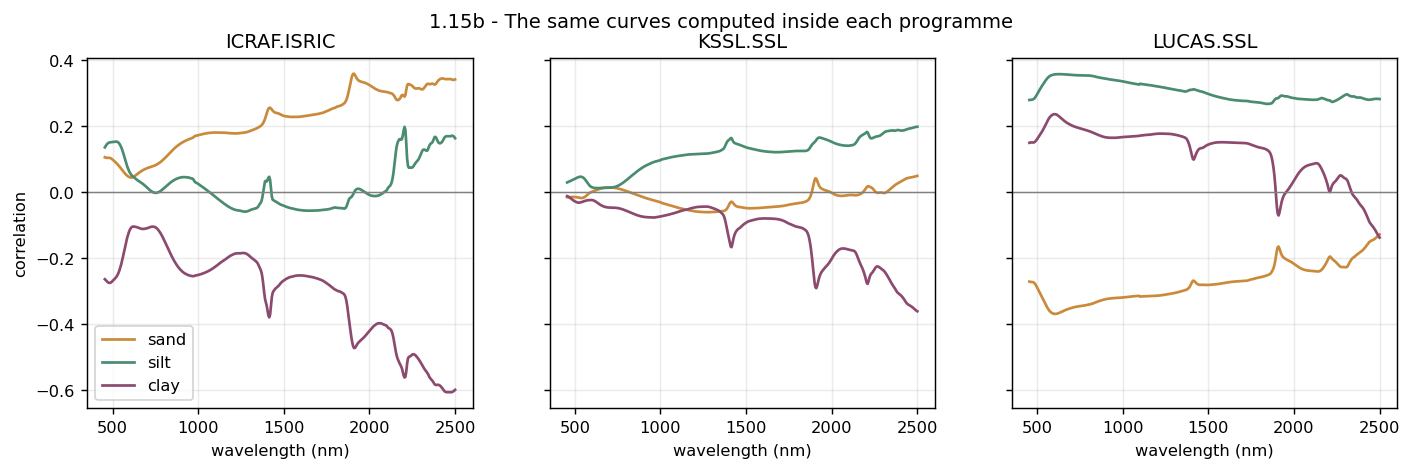
\includegraphics[width=0.92\textwidth]{figs/fig_1_15b.png}
\caption{Correlation between each wavelength and each target, computed inside each programme.
The three programmes do not agree. Clay is negative near 2475 nm inside ICRAF, but positive
near 605 nm inside LUCAS. When I pool the three programmes, these different relationships
cancel each other, and the pooled correlation falls to $|r| = 0.07$ for sand.}
\end{figure}

\begin{figure}[H]
\centering
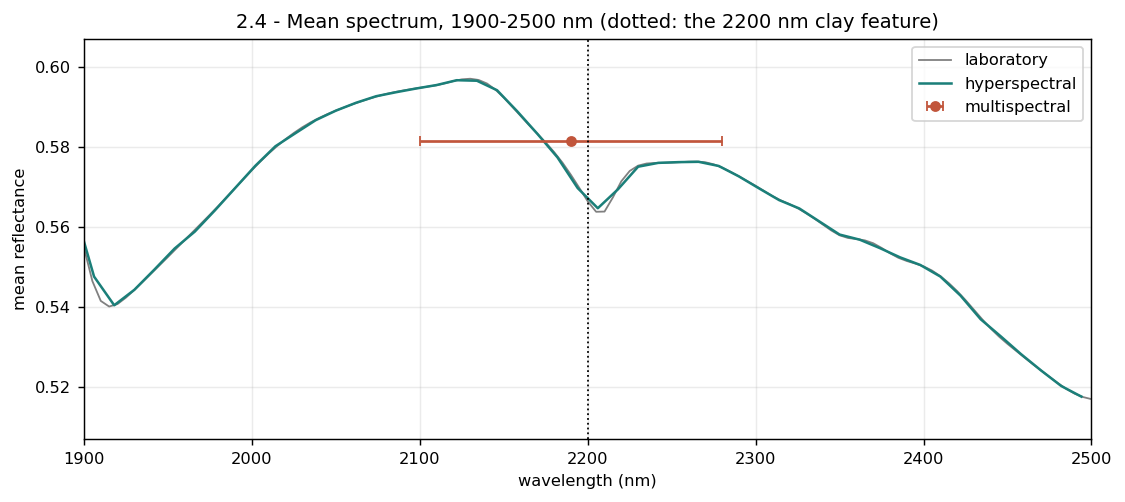
\includegraphics[width=0.62\textwidth]{figs/fig_2_4.png}
\caption{Mean spectrum between 1900 and 2500 nm, in the three versions. The grey and green
curves (laboratory and hyperspectral) both show the clay absorption near 2200 nm. The red
point is band B12, which is 180 nm wide. The dip and both of its sides are inside this single
band, so the average removes the feature. The depth of the feature goes from 0.0203 in the
laboratory, to 0.0167 in hyperspectral, and to exactly 0.0000 in multispectral.}
\end{figure}

\begin{table}[H]
\centering
\caption{$R^2$ for the nine configurations, under the two evaluations. The last column is the
difference. Every score under the second evaluation is negative, which means the model is
worse than simply predicting the average.}
\vspace{2mm}
\begin{tabular}{lrrr}
\hline
Configuration & Random split & One programme left out & Drop \\
\hline
Clay -- Laboratory spectrum & 0.544 & $-0.641$ & 1.185 \\
Clay -- Hyperspectral       & 0.539 & $-0.587$ & 1.126 \\
Clay -- Multispectral       & 0.273 & $-0.180$ & 0.453 \\
Silt -- Laboratory spectrum & 0.280 & $-2.193$ & 2.473 \\
Silt -- Hyperspectral       & 0.272 & $-2.091$ & 2.363 \\
Silt -- Multispectral       & 0.115 & $-0.014$ & 0.129 \\
Sand -- Laboratory spectrum & 0.333 & $-0.861$ & 1.194 \\
Sand -- Hyperspectral       & 0.326 & $-1.103$ & 1.429 \\
Sand -- Multispectral       & 0.101 & $-0.112$ & 0.213 \\
\hline
\end{tabular}
\end{table}

The table gives the main result of this lab. The mean drop from the random split to the
leave-one-programme-out evaluation is \textbf{1.174}. The mean drop from 410 laboratory
wavelengths down to 11 satellite bands is only \textbf{0.223}. So the way I evaluate the
model costs more than five times the sensor.

The table also shows something I did not expect. The richer version of the spectra transfers
worse. Clay loses 1.185 with the full spectra, but only 0.453 with 11 bands. Silt loses 2.473
against 0.129. With 410 wavelengths the model can learn the signature of each instrument and
use it as a shortcut. Eleven wide bands are too coarse for that.

\begin{figure}[H]
\centering
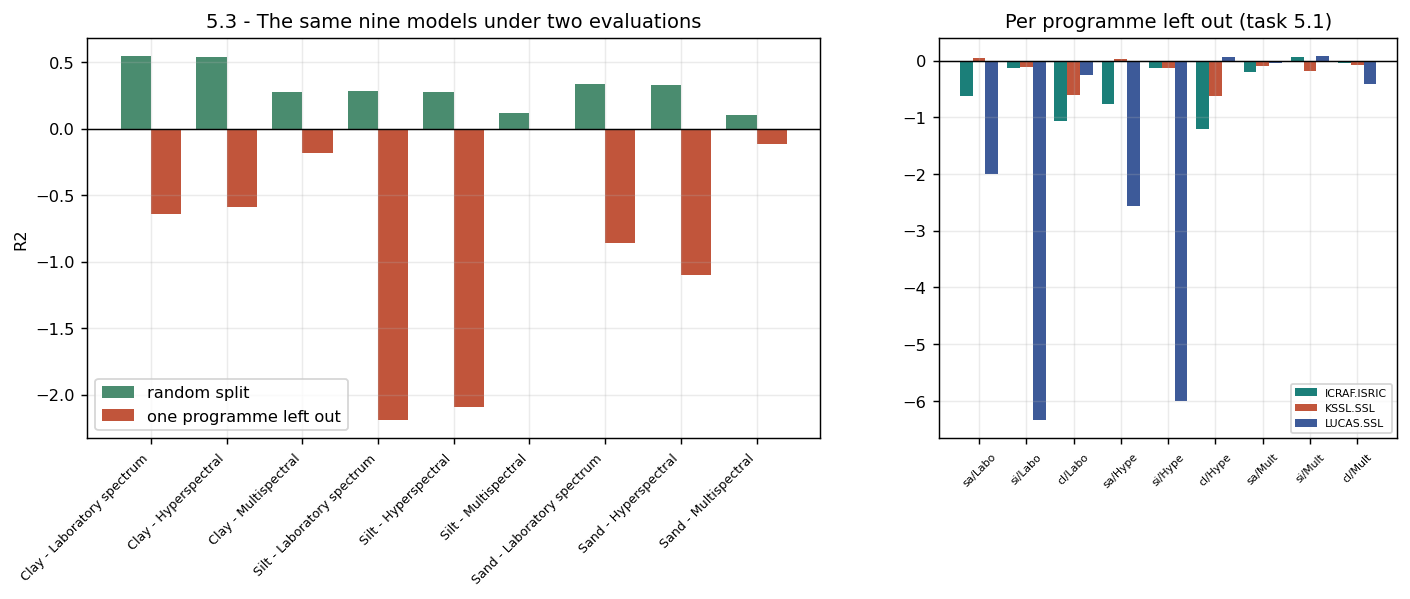
\includegraphics[width=0.92\textwidth]{figs/fig_5_3.png}
\caption{The same nine models under the two evaluations (left), and the score for each
programme that is left out (right). Green is the random split, red is one programme left out.
The right panel shows that the three folds are very different. Leaving out LUCAS gives a mean
$R^2$ of $-1.943$, but leaving out KSSL gives $-0.195$. Leaving out LUCAS also removes 55\% of
the training data, so this fold has two causes, not one.}
\end{figure}

\begin{figure}[H]
\centering
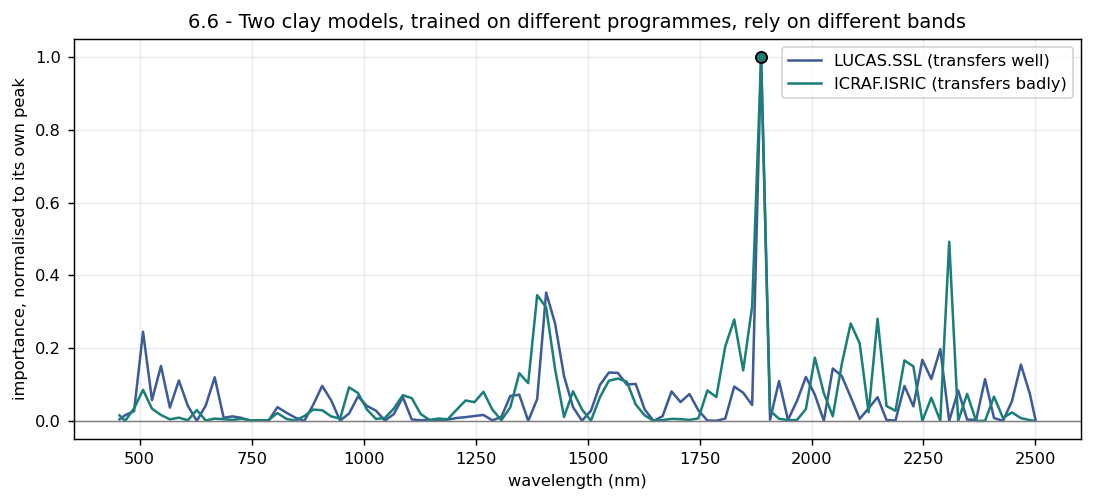
\includegraphics[width=0.60\textwidth]{figs/fig_6_6.png}
\caption{Importance profile of two clay models: one trained only on LUCAS, one trained only
on ICRAF. Each curve is divided by its own maximum, so I compare the shapes. The two profiles
agree ($r = 0.678$) and both peak on the same 20 nm block at 1888 nm. This is a water
absorption band. Clay controls how much water a soil holds, so this is an indirect clay
signal.}
\end{figure}

Figure 4 changes the explanation of the table. The two models do not use different
wavelengths. They use the same ones. So the problem is not which part of the spectrum the
model reads. The problem is the link between that signal and the clay value, and this link is
different for each instrument.

\section{Conclusion}

\textbf{What I found.} I can predict clay from a laboratory spectrum with $R^2 = 0.54$, silt
with 0.28 and sand with 0.33, using a random split. With 11 satellite bands these fall to
0.27, 0.12 and 0.10. But when I test on a survey that the model has never seen, every score
becomes negative. The evaluation scheme costs five times more than the sensor.

\textbf{What surprised me.} Three things. First, the richer version of the spectra transfers
worse, not better. Second, in task 3.3 I predicted that sand would be the hardest target. It
was, but only with 11 bands. With the full spectra silt is much worse, and it fails hardest
when a programme is left out. Third, I expected the two programme models to use different
wavelengths, because their correlation curves disagree. They use the same ones. A correlation
per wavelength and a fitted model do not measure the same thing.

\textbf{What I would do differently.} I would use the leave-one-programme-out evaluation from
the first day, not the random split. The random split gave scores that look reasonable and
are not true for a new survey. I would also treat the difference between instruments as the
main problem, not the model. Figure 4 suggests that a scatter correction, or one offset per
instrument, could help, because the models already look at the right place. Finally, I would
not mix three surveys without a plan: each model works better inside its own programme (0.645
for LUCAS, 0.650 for ICRAF) than the pooled model does across all three (0.544).

\end{document}
